\def\thesistitlefa{مدل محاسباتی همگام فدرالی براي شبکه‌هاي تطبیقی توزیع‌شده} ‌
\def\byfa{نگارنده:}
\def\authorfa{فاطمه بارانی}
\def\submitedforfa{رساله‌ی دکتری}
\def\undersupervisionfa{استاد راهنما:}
\def\supervisorfa{دکتر عبدالرضا سوادی}

\def\advisor{استاد مشاور :}
\def\advisorname{دکتر هادی صدوقی یزدی}

\def\datefa{1403}
\def\facultyfa{دانشکده مهندسی- گروه مهندسی کامپیوتر}
\def\universityfa{دانشگاه فردوسی }
\def\locationfa{مشهد}



\def\benamekhoda{به نام خدا}
\def\approvetitle{رساله دکتری}
\def\textonvan{عنوان}
\def\textnegaresh{نگارش}
\def\textexaminerscommittee{کمیته ممتحنین}
\def\textsupervisor{استاد راهنما}
\def\textinternalexaminer{استاد ممتحن داخلی}
\def\textexternalexaminer{استاد ممتحن خارجی}
\def\textsign{امضاء}
\def\textdate{تاریخ}

\def\textabstractfa{چکیده}
\def\textabstracten{Abstract}
\def\textkeywordfa{کلمات کلیدی}
\def\textkeyworden{Keywords}

\def\abstractfa{ 
در این رساله یک معماری سلسله مراتبی برای محاسبات کوانتومی توزیع شده ارائه شده است. در محاسبات کوانتومی توزیع شده، واحدها یا زیر سیستم‌ها از طریق پروتکل دورنوردی جهت انتقال اطلاعات کوانتومی با یکدیگر در ارتباط هستند. از آنجایی‌که دورنوردی کوانتومی نیاز به منابع کوانتومی و کلاسیک دارد، کاهش تعداد مورد نیاز این پروتکل در این سیستم‌ها از ضروریات می‌باشد. 

در این رساله یک بهینه سازی سلسه مراتبی دو سطحی جهت توزیع مناسب و متعادل کیوبیت‌ها بین زیر سسیتم‌ها ارائه شده است. 
در سطح اول، ابتدا مدلی ریاضی از مسئله‌ی افرازبندی مدار کوانتومی ارائه خواهد شد. سپس با تبدیل مدار کوانتومی به یک گراف تعداد برش کمینه جهت افرازبندی این مدار به $K$ زیر سیستم بدست خواهد آمد. تعداد برش‌های بدست آمده همان تعداد دروازه‌های سراسری بین سیستم‌ها خواهد بود. در این سطح، زمانبندی اجرای دروازه‌های کوانتومی در نظر گرفته نمی‌شود. خروجي اين سطح برچسب‌گذاري كيوبيت‌ها برحسب شماره افرازي است كه در آن قرار مي‌گيرند.

سپس در سطح دوم، با توجه به افرازبندی بدست آمده از سطح اول، در مرحله‌ی اجرای دروازه‌های سراسری کوانتومی، زمانی که یکی از کیوبیت‌های این دروازه از مبدا خود به مقصد مورد نظر دوربرد می‌گردد، ممکن است کیوبیت دوربري شده بتواند توسط تعدادی دروازه سراسری دیگر با رعایت محدودیت‌های پیش نیازی مورد استفاده قرار گرفته و در نتیجه موجب کاهش تعداد دورنوردی‌ها گردد.

در انتها جهت ارزیابی و مقایسه‌ی روش‌های پیشنهادی یا سایر الگوریتم‌ها، تعدادی معیار معرفی شد و الگوریتم پیشنهادی روی تعدادی مدار کوانتومی برگرفته از مجموعه‌ی مدارات کوانتومی تست و ارزیابی گردید. 
}

\def\keywordfa{ارتباطات سبز، زمان‌بندی خواب، پروتکل‌های مسیریابی، آگاهی از انرژی، بهینه‌سازی انرژی}

\def\abstracten{
Over recent years, green communications have been proposed as an emerging strategy to reduce the Carbon footprint produced by the networking sector. It consists in using different software and hardware techniques allowing to minimize the energy consumption of network components. A significant amount of energy saving can be obtained by switching redundant or unused network components to inactive mode, referred to as sleep-scheduling. To achieve this, the routing algorithm should aggregate traffic flows over a subset of network routers and their links, allowing other components to be switched off. The objective of this paper is to present a holistic survey on existing sleep-scheduling green routing protocols in wired networks. First, we propose a classification of main properties of green routing protocols and use the proposed classification to categorize and describe the existing literature. Moreover, we provide a comprehensive comparison of existing green routing protocols and determine the main characteristics, assets and issues of each proposal. Finally, we identify the open issues and key guidelines towards an ideal green routing protocol for wired networks.
\\

}
\def\keyworden{Terrain, Triangulated Irregular Network(TIN), Simplification, Weighted shortest path, Approximation algorithms, Heuristic algorithms}

%---------------------------
% بسم الله الرحمن الرحیم
\KashidaOff

\begin{titr}

{
\thispagestyle{empty}
$ $
\vskip 4cm
\begin{center}
\includegraphics*[width=0.6\textwidth]{besm.jpg}
\end{center}
}

%---------------------------
% Thesis Title Farsi
{
\thispagestyle{empty}
\begin{titlepage}
\begin{center}

\includegraphics[scale=0.4]{logo.png}\\
{\Large\facultyfa}
\vskip 1.5cm
{\large\bfseries\submitedforfa}
\vskip 1.5cm
{\Large\thesistitlefa}
\vskip 1.5cm

{\byfa}
\vskip 1.5cm
{\Large\bfseries\authorfa}
\vskip 2cm
{\undersupervisionfa}
\vskip 1cm
{\Large\bfseries\supervisorfa}
\vskip 3cm
{\advisor}
\vskip 1cm
{\Large\bfseries\advisorname}
\vskip 3cm
{\large\datefa}
\vskip 0.5cm
\end{center}
\end{titlepage}
}
\end{titr}



%%%%%%%%%%%\def\title{اظهارنامه(مربوط به انتشار رساله/پایان نامه)}
\def\tashakor{\large{تشکر و قدردانی}}
\def\date{تاریخ \quad امضای دانشجو}
\newpage
\baselineskip=0.75cm‎‎‎‎

\begin{center}
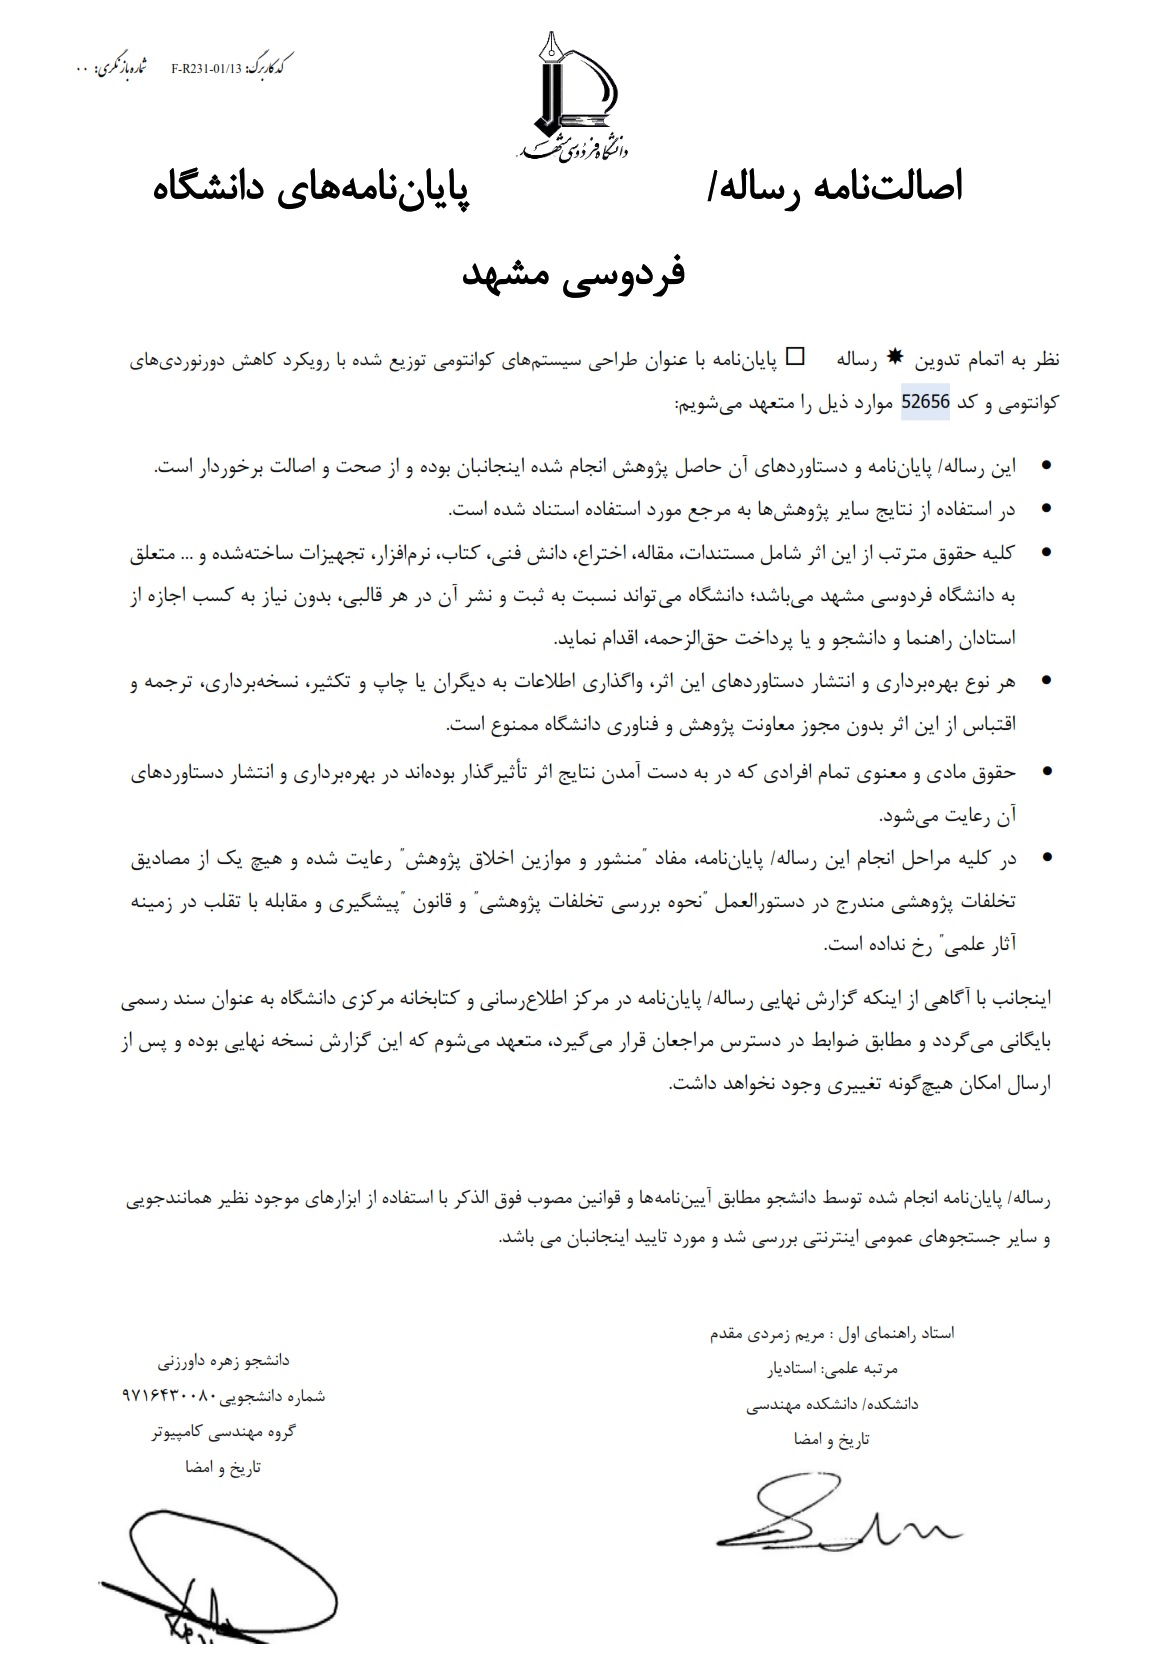
\includegraphics[scale=0.6]{esalat.jpg}\\
\end{center}
\newpage
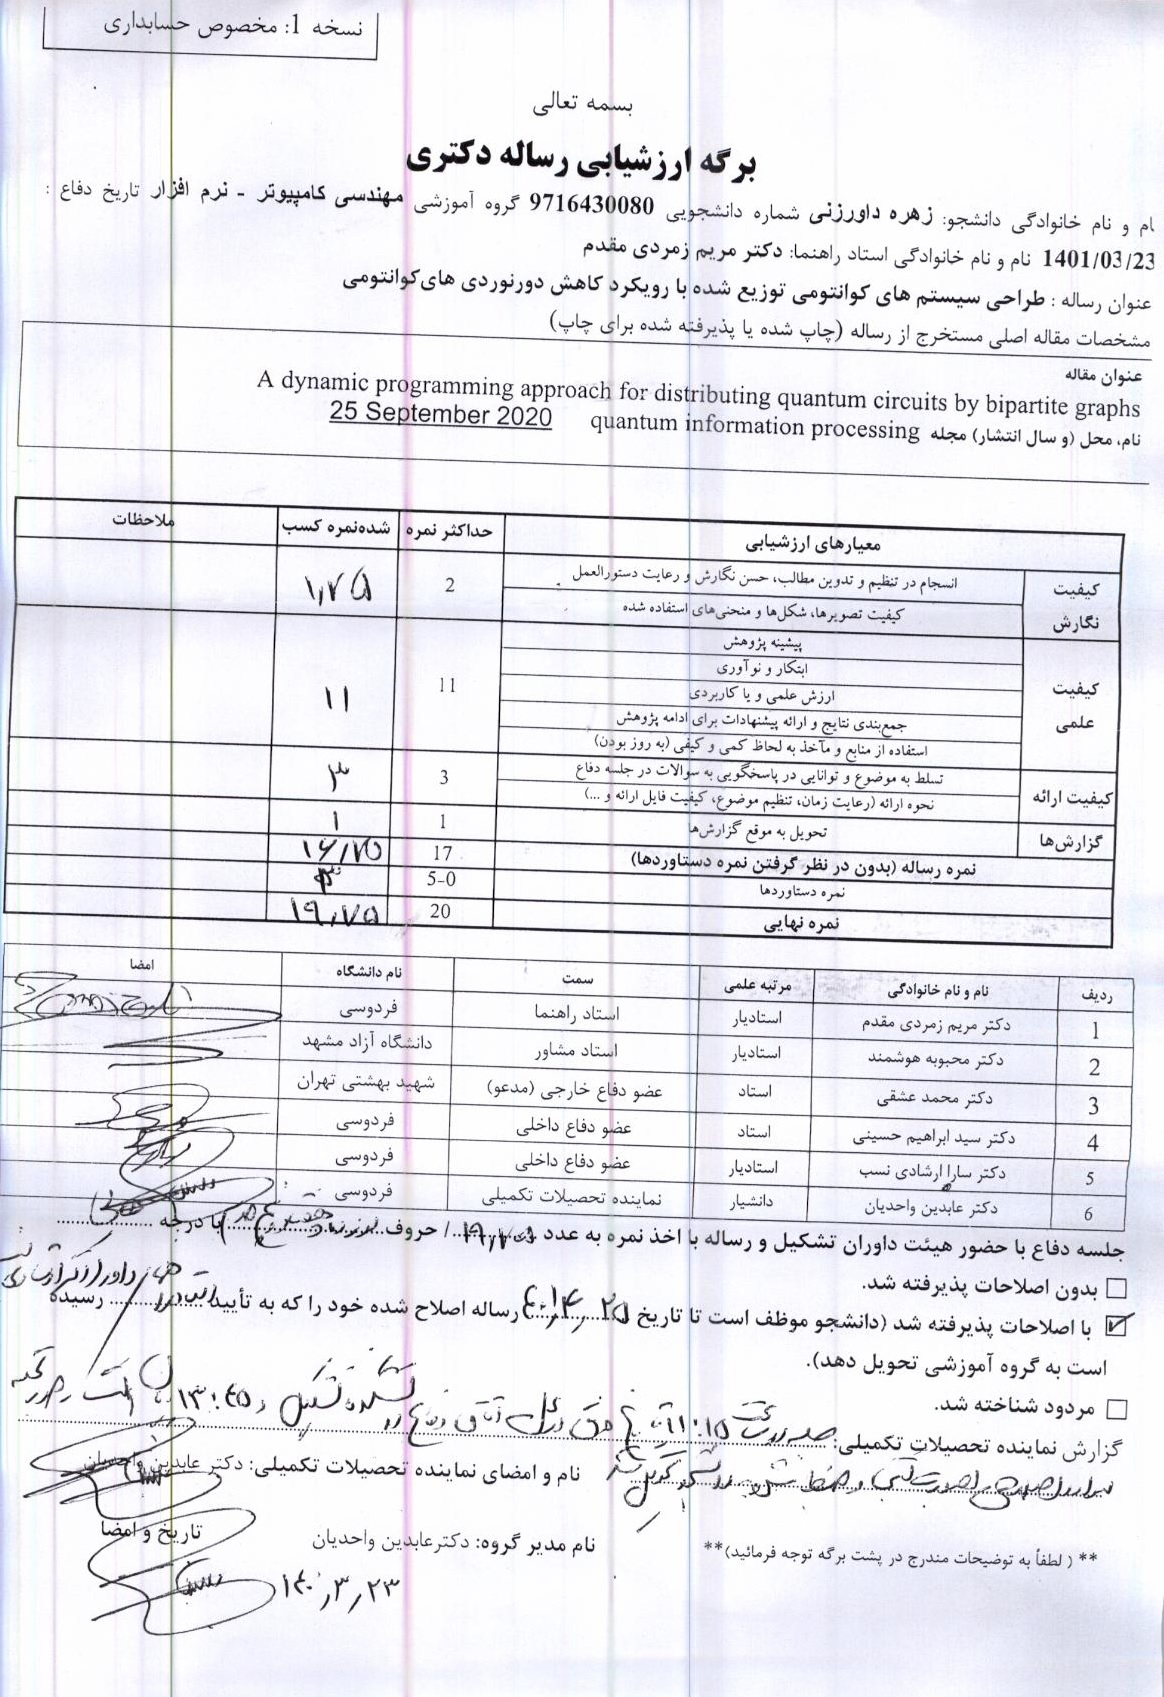
\includegraphics[scale=0.7]{arzesh.jpg}
\newpage
\KashidaOff
\begin{sols}

تقدیم به آنکه \\
\begin{center}
``تلاش مفهوم زندگی است'' 
\end{center}
\begin{flushleft}
را سرلوحه زندگی‌ام قرار داد.
\end{flushleft}

\end{sols}
\newpage
\begin{nazanint}
\begin{center}
\tashakor

منت خدای را عز و جل که طاعتش موجب قربت است و به شکر اندرش مزید نعمت.
\end{center}


در آغاز این رساله، بر خود می‌دانم از استاد بزرگوارم سرکار خانم دکتر مریم زمردی مقدم که با رهنمودهای ارزشمندشان همواره راهنما و چراغ راه من بوده‌اند، سپاس‌گزاری نمایم. حسن خلق، صبوری و همراهی این استاد گرانقدر همواره مایه‌ی آرامش و دلگرمی من در طول این دوره بوده است.

از سرکار خانم دکتر محبوبه هوشمند که با مشاوره‌های بسیار مفید و نکته‌های دلاویزشان راهگشای من در اتمام و اکمال این رساله بودند، تشکر نمایم.

همچنین، از سال‌ها زحمات و تلاش‌های بی‌دریغ کلیه اساتید محترم خویش در دانشگاه فردوسی مشهد که در تکوین دیدگاه من در دوره‌های کارشناسی، کارشناسی ارشد و دکتری نقش اساسی داشته اند، صمیمانه سپاس‌گزاری نمایم.

از پدر و مادر عزیزم، پشتیبان بی‌قید و شرط و همیشگی زندگی‌ام متشکرم.

از همسر مهربان و فرزند عزیزم که در این سال‌ها، پشتیبان، همراه و مشوق من بوده‌اند و این پژوهش بدون صبر و همراهی‌شان به سر انجام نمی‌رسید، سپاسگزارم. 
\end{nazanint}


\KashidaOn